\documentclass[12pt]{article}
\usepackage[hmargin=1in, vmargin=1in]{geometry}
\usepackage{fancyhdr}
\pagestyle{fancy}
\usepackage{lastpage}
\usepackage{graphicx}
\usepackage{listings}

\def\author{Mike Cooper}
\def\title{Milestone \#2 Report}
\def\date{\today}

\fancyhf{} % clear all header and footer fields
\fancyhead[LO]{\author}
\fancyhead[CO]{\title}
\fancyhead[RO]{\date}
% The weird spacing here is to get the spacing of \thepage to be right.
\fancyfoot[C]{\thepage\
                    / \pageref{LastPage}}

\setcounter{secnumdepth}{0}
\setlength{\parindent}{0pt}
\setlength{\parskip}{4mm}
\linespread{1.4}

\lstset{language=Python, basicstyle=\footnotesize, numbers=left}

\begin{document}

\subsection{Milestone Questions}
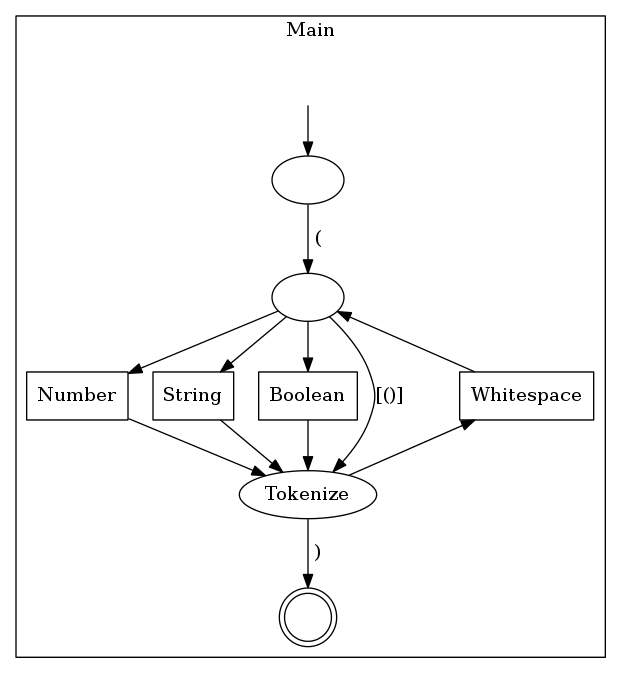
\includegraphics[height=3in]{main.png}
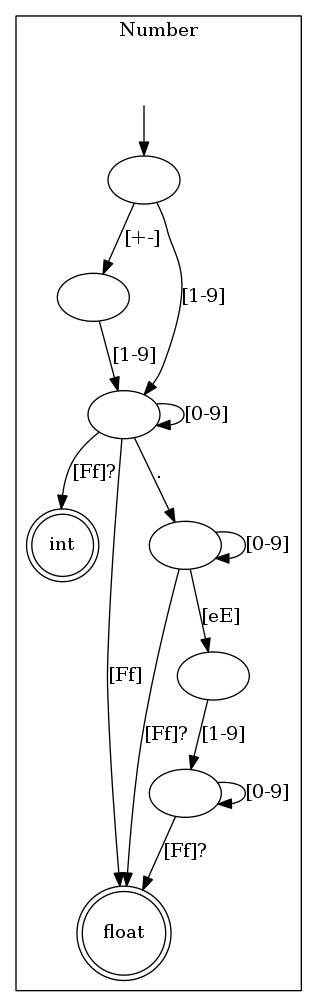
\includegraphics[height=4in]{number.png}

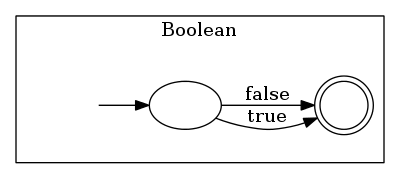
\includegraphics[height=1in]{boolean.png}
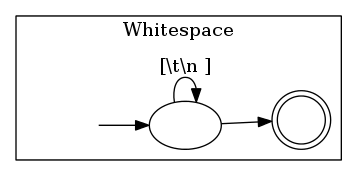
\includegraphics[height=1in]{whitespace.png}

\subsection{Specification}
This milestone is to teach us how to make a lexer, and so that we form a
formal specification of our language.

\subsection{Processing}
We designed a lexer and language together, by meeting together and drawing flow
charts and grammars on a whiteboard.

\subsection{Testing}
We tested the code by giving it sample bits of program at every step of the
design process, to test for validity, as well as giving it bad input to see how
it reacted.

\subsection{Retrospective}
I learned about parsing strings into tokens, and how to do real programming in
ruby. I also learned about working with my group members, and what the Symbol
Table is for.

\end{document}
